% Chapter 2 

\chapter{Dataset} % Main chapter title

\label{Chapter2} % For referencing the chapter elsewhere, use \ref{Chapter2} 

\lhead{Chapter 2. \emph{ Dataset }} % This is for the header on each page - perhaps a shortened title

%-----------------------------------------------------------------
BraTS(Brain Tumor Segementation has always been focusing on the evaluation of state-of-the-art methods for the segmentation of brain tumors in multimodal magnetic resonance imaging (MRI) scans. BraTS utilizes multi-institutional pre-operative MRI scans and focuses on the segmentation of intrinsically heterogeneous (in appearance, shape, and histology) brain tumors, namely gliomas. Furthemore, to pinpoint the clinical relevance of this segmentation task, BraTS also focuses on the prediction of patient overall survival, via integrative analyses of radiomic features and machine learning algorithms.

    \begin{figure}[h!]
        \centering
        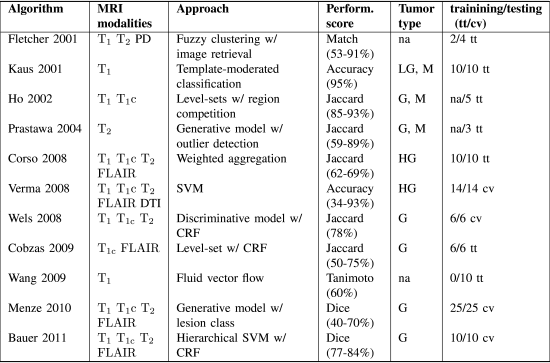
\includegraphics[scale=0.5]{Figures/dataset1.png}
        \caption[Dataset Description With Approaches]{Table I Data sets, MR image modalities, evaluation scores, and even tumor types used for self-reported performances in the brain tumor image segmentation literature differ widely. Shown Is a selection of algorithms discussed here and in [7]. Tumor type Is defined as g—glioma (unspecified), hg—high-grade glioma, lg—low-grade glioma, m—meningioma; “na” indicates that No information Is reported. When available the number of training and testing datasets Is reported, along with the testing mechanism: tt—separate training and testing datasets, cv—cross-validation}
        \label{fig:my_label}
    \end{figure}

   
\section{BraTS Dataset Annotations}
    
    BraTS images are available in .mha/nii(3d) format which we convert them to 2D images for deep learning processing. \\
    
    \begin{figure}[h!]
        \centering
        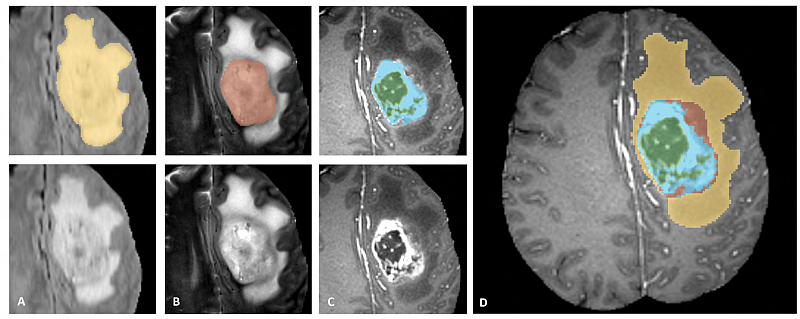
\includegraphics[scale=0.5]{Figures/BraTS_Tumors.png}
        \caption[BraTS Dataset Annotations]{Manual annotation through expert raters. Shown are image patches with the tumor structures that are annotated in the different modalities (top left) and the final labels for the whole dataset (right). Image patches show from left to right: the whole tumor visible in FLAIR (a), the tumor core visible in t2 (b), the enhancing tumor structures visible in t1c (blue), surrounding the cystic/necrotic components of the core (green) (c). Segmentations are combined to generate the final labels of the tumor structures (d): edema (yellow), non-enhancing solid core (red), necrotic/cystic core (green), enhancing core(blue)}
        \label{fig:BraTS_Dataset}
    \end{figure}
 
 

   
 \begin{table}[h!]
  \centering
  \caption{Types of brain MRI images}
    \begin{tabular}{|p{4cm}|p{3cm}|p{3cm}|p{3cm}|p{3cm}|}
       \hline
         \textbf{T1} & \textbf{T1c} & \textbf{T2} & \textbf{Flair} & \textbf{GT}\\
            \hline
            T1-weighted MRI & T1-enhanced weighted MRI & T2-weighted MRI & fluid-attenuated inversion-recovery MRI & Ground Truth\\
            \hline
        image contrast is based predominantly on the T1 (longgitudinal) relaxation time of tissue; tissue with short T1 relaxation time appears brighter & many tumors show signal enhancement after administration of contrast agent  & image contrast is based predominantly on the T2 (transverse) relaxation time of tissue; tissue with long T2 relaxation time appears brighter & bright signal of the CSF (cerebrospinal fluid) is suppressed which allows a better detection of small hyperintense lesions &  Actual region where the tumor is present \\
        \hline
            \end{tabular}
            
            \label{tab:my_label}
        \end{table}  
    
    
    
    